\documentclass[onecolumn, 12pt]{article}
\usepackage{fullpage}
\usepackage{graphicx}
\usepackage{cite}
\usepackage{amsmath}

\DeclareMathOperator{\URand}{U}
\providecommand{\ppos}{\ensuremath{\Vec{x}}}
\providecommand{\pvel}{\ensuremath{\Vec{v}}}
\providecommand{\gbest}{\ensuremath{\Vec{g}}}
\providecommand{\pbest}{\ensuremath{\Vec{p}}}
\providecommand{\constriction}{\ensuremath{\chi}}
\providecommand{\coeff}{\ensuremath{\phi}}
\newcommand{\bib}[1]{../../../bib/#1}

\topmargin .5in


\title{Improving Particle Swarm Optimization \\ in a Parallel World}
\author{Matthew Gardner}
\date{\today}

\begin{document}
\maketitle

\section{Introduction}
\label{sec:intro}

Optimization problems are ubiquitous in our modern world.  Businesses such as
Google need to decide where to place ads, scientists need to fit models to
data, and airlines need to schedule their flights.  All of those problems are
optimization problems, and optimization techniques can be used to find
solutions.  Optimization algorithms have been derived from all sorts of natural
phenomena.  Some methods look at the landscape of the function as they are
searching and follow hills to the best values, as in the gradient ascent
method.  Other methods take ideas from biology or metallurgy, like genetic
algorithms and simulated annealing.  Particle swarm optimization is a recently
developed optimization technique that draws on ideas from the sociology of
flocking birds.  

All of these methods, however, are fundamentally sequential in nature---they
need to be run in a specific order, and because of that, they are typically
only run on one machine.  The problems people want to solve are getting bigger,
and larger problems need to run on multiple machines in parallel.  Parallel
implementations of these algorithms have been attempted, but they do not often
perform as well as sequential versions for the amount of computation performed.
This work focuses on one of those algorithms, particle swarm optimization, and
improving its performance in a large-scale, parallel environment.  The work I
describe in Section~\ref{sec:topology} was done in collaboration with other
students I work with.  The work in Section~\ref{sec:specex} I did by myself.

The rest of this paper is outlined as follows.  In Section~\ref{sec:pso}, I
formally describe the particle swarm optimization algorithm, after giving a
brief description of optimization in general.  In Section~\ref{sec:topology},
I describe the sociological aspect of particle swarm optimization and
improvements that we have made for large swarms.  Section~\ref{sec:specex} then
introduces the idea of speculative execution in general and shows how it can be
done in particle swarm optimization.  I then conclude in Section~\ref{sec:conclusion}.

\section{Particle Swarm Optimization}
\label{sec:pso}

\subsection{Optimization in General}

The goal of optimization is to find the parameters to a function that either
maximize or minimize the function value.  To take an example from above, Google
needs to find the placements of website advertisements that generate the most
clicks for those websites.  In this example, the placements of advertisements
are the parameters to the function, and the number of clicks generated is the
function to be optimized.  A more mathematical example can be seen in
Figure~\ref{fig:cosine}.  The function shown has a point $x$ for which $f(x)$
is the highest.  Finding the precise location of that point is not a trivial
task, especially for more complicated functions, and it is that problem which
optimization techniques try to solve.

\begin{figure}
  \centering
  \includegraphics{cosine.eps}
  \caption{A complicated function: $\cos(x)\sin(10x)e^{-|x|}$}
  \label{fig:cosine}
\end{figure}

\subsection{Particle Swarm Optimization Specifically}

Particle swarm optimization was proposed in 1995 by James Kennedy and Russell
Eberhart.  It tries to intelligently search a multi-dimensional space by
mimicking the swarming and flocking behavior of birds and other
animals~\cite{kennedy-icnn95}. It is a sociological algorithm that depends on
interaction between particles to quickly and consistently find the optimal
solution to a problem.  The algorithm keeps track of a number of potential
solutions, called particles, which move somewhat randomly through the search
space at each iteration.  When the algorithm is done, the best position that
any of the particles ever found is returned.  Particles remember the best place
they have been, or solution they have evaluated, and when they move they are
attracted back to that place, as well as to the best solution other particles
have seen.  Specifically, the formulas for updating the position $\ppos_t$ and
velocity $\pvel_t$ of a particle at iteration $t$ are as follows:
\begin{align}
\label{eq:velupdate}
	\pvel_{t+1} &=
		\constriction \left[ \pvel_t +
			\coeff_1\URand()\otimes(\pbest - \ppos_t) +
			\coeff_2\URand()\otimes(\gbest - \ppos_t)
		\right] \\
\label{eq:posupdate}
	\ppos_{t+1} &= \ppos_t + \pvel_{t+1}
\end{align}
where \( \URand() \) is a vector of random numbers drawn from a uniform
distribution, the \( \otimes \) operator is an element-wise vector
multiplication, $\pbest$ (called pbest) is the best position the current
particle has seen, and $\gbest$ (called gbest) is the best position any of the
other particles have seen.  \( \coeff_1 \), \( \coeff_2 \), and \(
\constriction \) are parameters with prescribed values required to ensure
convergence (2.05, 2.05, and .73,
respectively)~\cite{clerc-tec02}~\cite{poli-aea08}.

The sociology in this algorithm defines which other particles form the
``neighborhood'' of a given particle---the other particles whose best solution
it sees (again, that is $\gbest$ in the equations above).  If particle 1 is a
neighbor of particle 2, then particle 1 will be influenced by good values that
particle 2 sees.  But if particle 3 is not a neighbor of particle 1, particle 1
will be completely unaware of good values that particle 3 finds.  

There are many ways to define a particle's neighborhood, varying from the
entire rest of the swarm to just one other particle.  

The way a neighborhood is defined can have drastic effects on the performance
of the algorithm; the more neighbors each particle has, the faster information
spreads throughout the swarm, and the quicker the algorithm converges.  For
some problems it is possible that the algorithm converges too quickly and gets
caught in a local optimum; it stops on a hill when there is a mountain next to
it.  For those kinds of problems, less communication, or smaller neighborhoods,
is often preferable.

\section{Topology in PSO}
\label{sec:topology}

Much work has been done on the sociological aspect of particle swarm
optimization, trying to determine the best neighborhood structure to use for
various classes of problems.  That work focused on swarms of tens of particles
to several hundred particles on a single machine.  Conclusions were reached
about which neighborhood structures worked best, but only in this limited
context~\cite{bratton-sis07}.  With the advent of parallel processing and the
potential to have swarms of thousands or hundreds of thousands of particles,
some of the earlier work needs rethinking.  This section focuses on
neighborhood structures in very large swarms, especially when the algorithm is
run in parallel on multiple machines.  

\subsection{Defining Topology}

Many different neighborhood structures have been proposed and
tested~\cite{kennedy-cec02}.  In the literature, neighborhood structures are
referred to as topologies.  Two of them are more common---the complete or gbest
topology, where all particles communicate with all other particles, and the
ring or lbest topology, where each particle only communicates with its two
immediate neighbors~\cite{bratton-sis07}.  

To formalize the description of topologies, we can consider the swarm as a
graph $\{V,E\}$, where the set of particles forms the nodes $V$ on the graph
and the (directed) edges $E$ between nodes represent communication between
particles.  If (1,2) is an edge in the graph, then particle 1 influences
particle 2's gbest, or particle 1 is in particle 2's neighborhood.  The
neighborhood $N_i$ of particle $i$ can be written formally as 
\[N_i = \{p_j|(j,i)\in E\}\]

Neighborhoods can also be thought of in terms of which other particles a
particular particle sends its information to, instead of which ones it gets
information from.  This conceptualization makes the communication a little bit
more explicit (and more directly relates to how to actually run the algorithm)
and will be used to describe topologies throughout the rest of this paper.
$N_i$ then becomes
\[N_i = \{p_j|(i,j)\in E\}\]

The two topologies mentioned previously, complete and ring, would then have the
following neighborhoods for each particle $i$ in a swarm of $n$ particles:
\[\mathrm{Complete:}\ N_i = \{1,2,3,\dots,n\}\]
\[\mathrm{Ring:}\ N_i = \{i-1,i,i+1\}\]

For the benefit of more visual readers, the two topologies are shown in graph
form in Figure~\ref{fig:topgraphs}; notice how many more lines are in the 
complete topology than in the ring topology.

\begin{figure}
  \centering
  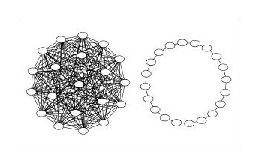
\includegraphics{gbest_and_lbest.eps}
  \caption{The complete and ring topologies in graph form.  Figure taken from
  tracer.uc3m.es/tws/pso/neighborhood.html.}
  \label{fig:topgraphs}
\end{figure}

\subsection{Which Topology to Use}

There is a theorem about optimization called ``No Free Lunch''
\cite{wolpert-tec97}. In essence it says that no optimization algorithm can do
better than any other optimization algorithm across all functions.  If you do
better on some functions with a given algorithm that is because you do worse on
other functions.  This applies directly to the question of which topology in
PSO is the ``best,'' because it proves that there really is no ``best''
topology across all functions.  When selecting a topology you must have a
specific type of function in mind, and pick the topology that works best for
that type of function.

An interesting question along those lines is, ``Are the problems that most
people are interested in solving inherently similar?''  If that is the case,
one could design an algorithm that performs better on the problems people care
about, taking a performance hit only on functions that don't matter anyway.
But, because of No Free Lunch, any argument claiming that a particular
algorithm or topology is better than another must make that claim only for a
specific set of functions.

When deciding which topology to use, then, making a wise decision requires
having a certain kind of function in mind.

The complete topology is often preferable for many problems, because it allows
information to be shared quickly throughout the swarm and helps the algorithm
converge more quickly.  However, too much shared information can cause
premature convergence, as mentioned previously, so some researchers are wary of
the complete topology.  In the absence of knowledge about the function to be
optimized, researchers recommended, the ring topology should be used.  It might
take longer, but at least it won't get stuck, they say \cite{bratton-sis07}.

\begin{figure}
  \centering
  \includegraphics{iters_rast.eps}
  \caption{PSO performance on the function Rastrigin with varying numbers of
  particles.}
  \label{fig:rast}
\end{figure}

For a swarm of 50 particles it is accurate that complete often doesn't perform
well, and most researchers were satisfied to stop with a swarm that size.  We
have shown, however, that increasing the number of particles in a swarm will
help the algorithm avoid premature convergence, making complete the best
topology even for somewhat complicated functions~\cite{mcnabb-cec09}.
Figure~\ref{fig:rast} shows the performance of PSO on a commonly used benchmark
function, the Rastrigin function, with varying numbers of particles.  Notice
that with 50 particles the algorithm does get stuck pretty early, not finding
significantly better values after 250 iterations.  This is precisely what many
researchers in the field were saying.  With more particles, however, the
algorithm finds much better values and continues to find better values well
past 250 iterations.

\subsection{Communication Overhead}

In a parallel system, another problem with the complete topology is that
communication between processors is expensive relative to the amount of time it
takes to evaluate the functions many people work with.  A quick look at
Figure~\ref{fig:topgraphs} shows the incredibly large number of messages that
need to be sent between particles for a relatively small swarm.  Communicating
all of the information from every particle at every iteration can take orders
of magnitude more time than doing a simple evaluation and render
parallelization of the algorithm worthless.  

We developed a modification to the algorithm along with a new topology that
approximates the complete topology with much less communication.  If each
particle at each iteration randomly chooses a small set of particles to send
its information to, eventually information will be communicated throughout the
whole swarm.  We call this the Random topology, and it is formally defined as
follows:
\[\mathrm{Random:}\ N_i = \{i,U_1,U_2,\dots,U_k\}\]
where $U_j$ is a random number from 1 to $n-1$, and $k$ is the number of 
neighbors to send information to at each iteration.

In the standard particle swarm optimization algorithm, the best neighbor that a
particle is attracted to (the \gbest in the formula above) is taken from its
current neighborhood.  With the random topology we proposed, particles can get
confused, being attracted to a different neighbor at every iteration, and
performance significantly decreases.  We modified the algorithm slightly such
that each particle remembers the best neighbor it has ever had and is attracted
to that position instead of its current best neighbor.  Using this modification
and a random topology, we saw performance that was indistinguishable from
complete with only 5\% of the communication, and the speed up is significant
even in a serial implementation~\cite{mcnabb-cec09}.  

Figure~\ref{fig:rastrand} shows the performance of Random versus Complete on
the function Rastrigin for various swarm sizes.  The x-axis shows the number of
particles in the swarm, and the y-axis shows the best function value found
after 500 iterations.  It can be seen from the graph that Random does a very
good job at approximating the Complete topology while required only a small
fraction of the communication.

\begin{figure}
  \centering
  \includegraphics{randstar.eps}
  \caption{Random with various amounts of communication versus the Complete
  topology on the function Rastrigin.}
  \label{fig:rastrand}
\end{figure}

\subsection{Subswarms}

We have run all of the experiments I've talked about so far with swarms of up
to 4000 particles.  All of them were run with a serial implementation of
particle swarm optimization on a single machine, though the results can be used
in designing parallel algorithms.  With more than 4000 particles the algorithm
becomes very computationally expensive on a single machine.  We have
implemented a parallel version of particle swarm optimization using Google's
MapReduce framework for parallel computation~\cite{dean-osdi04}.  Soon we will
have it working well enough to run swarms of hundreds of thousands of particles
on hundreds of machines at a time, and we will further explore the issues
involved with parallel particle swarm optimization.  

Many new possibilities for topologies arise when the algorithm is run in
parallel with large swarms.  We have proposed, but not yet fully tested, a
topology of subswarms, where each of a hundred machines would evaluate 500 or
1000 particles and send only its best value to all other machines, drastically
reducing the amount of inter-processor communication.  In our formal notation,
the subswarms topology can be described as

\[\mathrm{Subswarms:}\ N_i = \{j|j\%k = i\%k\}\]
where $k$ is the number of subswarms in the swarm, and \% is the mod operator.
For a small example, in a swarm of 12 particles with 3 subswarms, the sets of
neighbors would be \{1, 4, 7, 10\}, \{2, 5, 8, 11\}, and \{3, 6, 9, 12\}.

Our preliminary results show that this approach is very
promising~\cite{mcnabb-cec09}.  Figure~\ref{fig:subswarms} shows the results
of using the Subswarms topology with 400 particles in each swarm, versus just
using 400 particles in a Complete topology.  Subswarms clearly outperforms
Complete in this case.

\begin{figure}
  \centering
  \includegraphics{islands_iters_rast.eps}
  \caption{Subswarms versus Complete topologies on the function Rastrigin.}
  \label{fig:subswarms}
\end{figure}

\section{A Different Speed up---Speculative Execution}
\label{sec:specex}

\subsection{Speculative Exectuion in General}

Speculative execution in a program is the execution of code that may or may not
end up actually being needed.  Modern processors routinely do this when a
conditional branch is encountered---they try to predict which branch will
end up being needed and continue their execution.  If it turns out that the
prediction was incorrect, the work is discarded.  But if the prediction was
right, the program can execute much faster than if it had waited on the branch.  

\subsection{Speculative Execution in Particle Swarm Optimization}

In many optimization algorithms speculative execution is impossible, because
the next iteration of the algorithm depends on the evaluation of the function
during the previous iteration.  To know which positions to speculatively
evaluate you have to already have evaluated the current position, and then it's
not speculative anymore.  In simulated annealing, for instance, the probability
of accepting a new position depends on the difference in function value between
the new position and the current one.  In gradient descent, the gradient of the
function must be determined (which includes actually evaluating it) to know how
far to move before sampling the function again.  It may be possible to modify
these algorithms to allow for speculative execution, but their standard
executions cannot be done speculatively.

Particle swarm optimization is rather unique in that it does not require the
evaluation of the function to know what the next position of each particle will
be.  It simply depends on \emph{which} particle ended up having the best
position and whether or not the current particle found a better spot than it
had seen before.  That means you can just compute all possible next
positions---all combinations of which particle is the new gbest and whether or
not pbest was updated (\gbest\ and \pbest\ from equation
\eqref{eq:velupdate})---and evaluate each position in parallel.  That computes
two iterations at the same time.  

\subsection{Is is worth it?}

Speculative execution uses a lot of extra work to compute two iterations at the
same time, but for some functions performing more iterations makes more
progress than adding extra particles.  The No Free Lunch theorem again shows
its head here, though, because if you do better with one algorithm on a certain
function or set of functions, that's because you do worse on other functions.
There are, however, a set of functions that do better with more iterations than
with more particles.

\begin{figure}
  \centering
  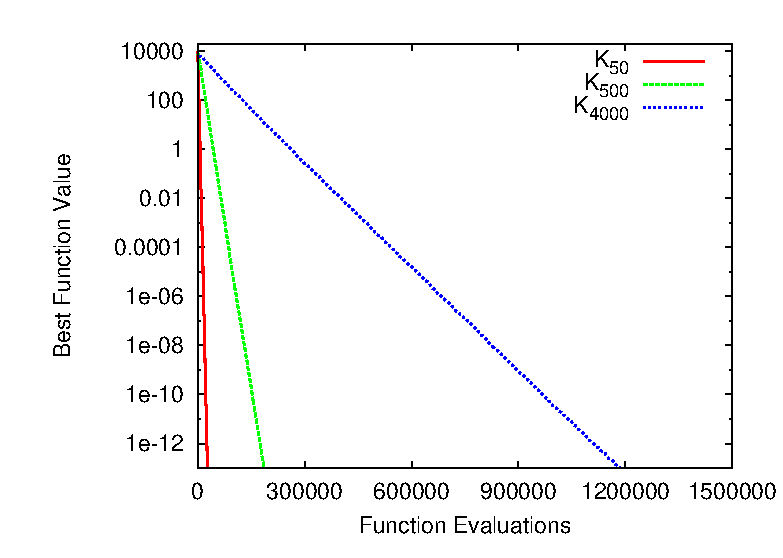
\includegraphics{evals_sphere.eps}
  \caption{Best value found on the function Sphere versus the number of 
  function evaluations with varying swarm sizes.}
  \label{fig:sphere}
\end{figure}

Figure~\ref{fig:sphere} shows an example of this: the function Sphere.  The
graph shows the best function value found over a number of function
evaluations.  This is different than previous graphs that have shown function
value against a number of iterations.  At each iteration, a swarm of 50
particles performs 50 function evaluations, where a swarm of 4000 particles
performs 4000 evaluations.  Figure~\ref{fig:sphere} shows that the extra 3950
function evaluations spent on the extra particles in a 4000 particle swarm
really don't do any good.  It would be more worth it to just do more iterations
of a 50 particle swarm than to have a swarm of 4000 particles.

The benefit of adding more particles comes in when you have hundreds or
thousands of processors in a parallel cluster.  You can't use 4000 machines to
run a swarm of 50 particles---3950 of the processors would be idle the whole
time.  Adding more particles to the swarm then improves performance without
adding any extra time (ignoring inter-processor communication cost for the
moment).  But for some functions, a better idea than using the extra 3950
processors to add more particles to the swarm is to use the processors
speculatively so that two iterations can be done at the same time.
Figure~\ref{fig:sphere} shows just one example of a function that would be
better optimized by performing speculative execution than by adding extra
particles.



\section{Conclusion}
\label{sec:conclusion}

In a world where people are swimming in processing power, many old algorithms
need to be rethought.  Parallel computing architectures allow for new
techniques that were previously impossible.  In the realm of optimization,
particle swarm optimization is uniquely capable of reaping great benefits from
parallel processing.  I have reviewed just a few ways in which PSO can be
improved to harness the increased power of parallel clusters.  As more
researchers tackle the problems of modifying and adapting algorithms to better
utilize the resources that are now available, our ability to solve problems
with computers will increase dramatically.


\bibliographystyle{plain}
\bibliography{%
\bib{pso/kennedy-icnn95},%
\bib{pso/clerc-tec02},%
\bib{pso/poli-aea08},%
\bib{pso/topology/kennedy-cec02},%
\bib{pso/bratton-sis07},%
\bib{aml/mcnabb-cec09},%
\bib{mapreduce/dean-osdi04},%
\bib{wolpert-tec97}}

\end{document}
